\problemname{Mountain Allocation}

\noindent The Danes are envious that all other countries have much better ski slopes. 
The issue has been brought all the way to the European Court of Justice,
and it has been decided that the borders of European countries should be redrawn so that the distribution
of ski slopes is as fair as possible. Europe can be modeled as a grid of size $R \times C$,
where the cell at row $i$, column $j$ has a number $m_{ij}$ indicating 
how many mountains are in that cell.
A country consists of a contiguous collection of cells,
where the total number of mountains in the country divided by the area of the country
determines how pleasant it is to ski there.
A country is contiguous if it is possible to move within the country
from each cell to every other cell, by moving only in the four cardinal directions (i.e., not diagonally).
Help the Danes to divide Europe into $N$ countries so that 
the mountains are distributed as evenly as possible relative to the countries' areas!

\section*{Input}
The first line contains the integer $T$, the number of the testcase.
The second line contains three integers $R$, $C$ ($2 \le R \times C \le 10^5$), and $N$ ($1 \le N \le 16000$), 
representing the number of rows and columns in the grid,
and the number of countries, respectively.
Then, there are $R$ lines, one for each row in the grid. 
Each row contains $C$ numbers. In row $i$, column $j$ 
the number $m_{ij}$ ($0 \leq m_{ij} \leq 1000$) represents 
the number of mountains at the corresponding location in the grid.

\section*{Output}
The $N$ countries are numbered from $0$ to $N - 1$. Print $R$ rows with $C$ numbers each, where each number indicates
the country number that owns the cell after your division.

\section*{Points}
Your solution will be tested on 10 test cases,
each of which can earn up to 10 points.
Let $a_k$ be the total number of mountains in country $k$ divided by the number of cells in the country,
and let $\bar{a}$ be the total number of mountains divided by the total number of cells in the entire grid.
You want to minimize the value of the expression

\[
S = \sum_{k=1}^{N}{(a_k - \bar{a})^2}.
\]

\noindent If $S = 0$, your solution will earn 10 points for the test case.
Otherwise, your score is determined by the expression

\[
10 \times \max(1, \frac{S_D}{S}),
\]

\noindent where $S_D$ is what the judge's solution achieved on the same test case.

\noindent
\begin{tabular}{| l | l | p{12cm} |}
  \hline
  \textbf{Group} & \textbf{Point value} & \textbf{Constraints} \\ \hline
  $1$    & $10$      & $R = C = N = 10$ \\ \hline
  $2$    & $10$      & $R = 1$, $C = 100000$, $N = 1000$ \\ \hline
  $3$    & $10$      & $R = 2$, $C = 10000$, $N = 1000$ \\ \hline
  $4$    & $10$      & $R = C = 200$, $N = 40$, $m_{ij} = 0$ or $m_{ij} = 1$ for all $i$, $j$ \\ \hline
  $5$    & $10$      & $R = C = 50$, $N = 250$ \\ \hline
  $6$    & $10$      & $R = C = 200$, $N = 2$ \\ \hline
  $7$    & $10$      & $R = C = 200$, $N = 400$ \\ \hline
  $8$    & $10$      & $R = C = 400$, $N = 16000$ \\ \hline
  $9$    & $10$      & $R = C = 400$, $N = 1600$ \\ \hline
  $10$    & $10$      & $R = C = 400$, $N = 1600$ \\ \hline
\end{tabular}


\section*{Explanation of Sample 1}
\begin{figure}[!h]
  \centering
  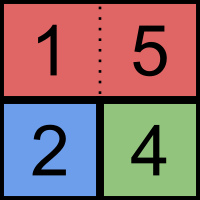
\includegraphics[width=2cm]{sample1.png}
  \quad
  \caption{Division of countries in Sample 1.}
\end{figure}

\noindent In the first sample, $\bar{a} = \frac{1 + 5 + 2 + 4}{4} = 3$. The average values are 3 for the red country, 2 for the blue country, and 4 for the green country. This gives $S = 2$.

\section*{Explanation of Sample 2}
\begin{figure}[!h]
  \centering
  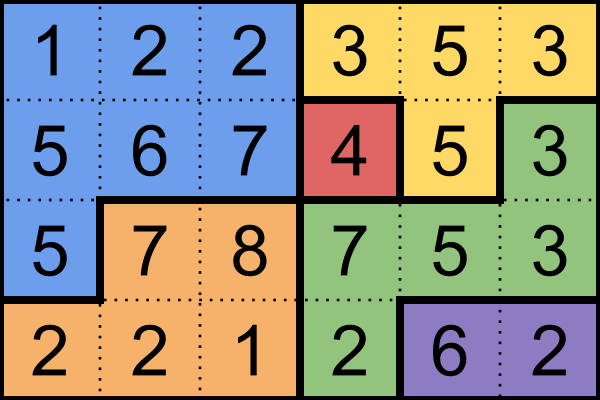
\includegraphics[width=5cm]{sample2.png}
  \quad
  \caption{Division of countries in Sample 2.}
\end{figure}

\noindent In the second sample, $\bar{a} = 4$. The average value in each country is 4. This gives $S = 0$, which is a perfect solution.
